\documentclass[11pt,a4paper]{article}
\usepackage[utf8]{inputenc}
\usepackage{geometry}
\geometry{a4paper, margin=1in}
\usepackage{graphicx}
\usepackage{hyperref}
\usepackage{amsmath}
\usepackage{booktabs}
\usepackage{cite}
\usepackage{float}
\usepackage{caption}
\usepackage{subcaption}
\usepackage{tikz}
\usetikzlibrary{shapes.geometric, arrows.meta, positioning, fit, calc, backgrounds}
\usepackage{setspace}
\usepackage{tabularx}
\usepackage{listings}
\usepackage{color}

\title{\textbf{Cardio-Sahayak India: A Multimodal Foundation Model for Complex Cardiology Care in South Asian Populations}}
\author{
@tp53(ashish makani) \\
\texttt{spiff007@gmail.com} \\
\texttt{github.com/inventcures/cardio-sahayak}
}
\date{March 2026}

\begin{document}
\setstretch{1.15}

\maketitle

\begin{abstract}
The scarcity of specialized cardiovascular medical expertise poses a severe challenge to global healthcare delivery, a problem acutely felt in India where the burden of cardiovascular disease (CVD) is growing rapidly. Furthermore, South Asian populations present unique clinical phenotypes, such as lower BMI thresholds for myocardial infarction and specific genetic predispositions (e.g., the MYBPC3 $\Delta$25bp variant). General-purpose medical AI models often overlook these population-specific nuances. In this preprint, we introduce \textbf{Cardio-Sahayak India}, an open-source, dual-architecture Large Language Model (LLM) and Vision-Language Model (VLM) explicitly fine-tuned for complex cardiology care in the Indian demographic. 

Building upon the MedGemma-27B backbone and the MedSigLIP vision encoder, we outline a novel two-phase fine-tuning methodology. In Phase 1, the model learned general medical reasoning. In Phase 2, we introduced a rigorously curated 166-record \textit{V2 Dataset} integrating Indian clinical notes (EkaCare), Gemini-driven synthetic phenotype shifts, and multimodal scanned ECG references (IIIT-Hyderabad, ScienceOpen). By executing a Quantized Low-Rank Adaptation (QLoRA) process on serverless A100 GPUs and patching the model architecture for GGUF compatibility, we successfully converted the entire 27-billion parameter framework into highly quantized, offline-ready artifacts. Cardio-Sahayak India democratizes subspecialist-level cardiac care, bringing culturally and genetically contextualized AI directly to resource-constrained edge clinics across the subcontinent.
\end{abstract}

\newpage

\section{Introduction}

Cardiovascular diseases (CVD) have firmly established themselves as the leading cause of mortality in India, accounting for over a quarter of all deaths in the country. A distinct and alarming epidemiological pattern has emerged in the subcontinent: Myocardial Infarction (MI) and other severe cardiac events in South Asian populations often occur 5 to 10 years earlier than in Western demographics. This divergence in presentation is widely recognized in clinical literature as the "South Asian Phenotype."

\subsection{The South Asian Phenotype}
The South Asian Phenotype is characterized by a complex interplay of genetic, metabolic, and environmental factors. Unlike typical Western presentations, South Asian patients frequently exhibit central adiposity and insulin resistance despite presenting with "normal" standard body mass indices (BMIs). Western clinical algorithms, which heavily rely on generic BMI thresholds, systematically underestimate the cardiovascular risk in this population. 

Furthermore, specific genetic markers compound this risk. Most notably, the MYBPC3 $\Delta$25bp variant---a 25-base-pair deletion in the cardiac myosin binding protein C gene---is strongly linked to an increased risk of developing heart failure and hypertrophic cardiomyopathy (HCM). This specific variant affects approximately 4\% of the Indian population, translating to an estimated 45 million individuals. Despite the vastness of this vulnerable cohort, general-purpose medical AI diagnostic tools are trained predominantly on Western datasets (such as MIMIC and proprietary US hospital records), leading to a critical gap in personalized, culturally, and genetically sensitive care.

\subsection{The Workforce Crisis and AI as a Solution}
Compounding the biological and genetic challenges is a severe structural deficit in the healthcare system. The ratio of specialized cardiologists to the general population in India is critically low, particularly in rural and semi-urban settings. Primary care physicians and general practitioners are frequently the first line of defense for complex cardiac presentations, yet they lack the subspecialty training required to navigate intricate genetic cardiomyopathies or subtle ECG abnormalities that precede catastrophic events.

To address these disparities, we developed \textbf{Cardio-Sahayak India}, an advanced multimodal diagnostic assistant tailored specifically for the South Asian demographic. Cardio-Sahayak operates as a "cognitive offloader" and expert assistant for general practitioners, effectively bringing a virtual subspecialist to the point of care.

\section{Methodology: A Two-Phase Training Approach}

To accommodate both text-based clinical reasoning and raw diagnostic imaging (12-lead ECGs), Cardio-Sahayak employs a dual-architecture design based on \texttt{google/medgemma-27b-it} and the \texttt{google/medsiglip-448} vision encoder. Training was split into two distinct phases to prevent catastrophic forgetting while injecting highly specific demographic knowledge.

\subsection{Phase 1: General Medical Reasoning}
The initial phase utilized standard Supervised Fine-Tuning (SFT) over 3 epochs with a learning rate of $2\times 10^{-4}$. This phase aligned the MedGemma backbone with general cardiology guidelines and established the Multimodal Electrocardiogram Instruction Tuning (MEIT) framework to fuse visual embeddings from MedSigLIP into the LLM's latent space.

\subsection{Phase 2: The V2 Dataset \& South Asian Contextualization}
To address the critical data drought in South Asian cardiology, we engineered a highly specialized \textit{V2 Dataset} comprising 166 complex records.

\begin{figure}[H]
    \centering
    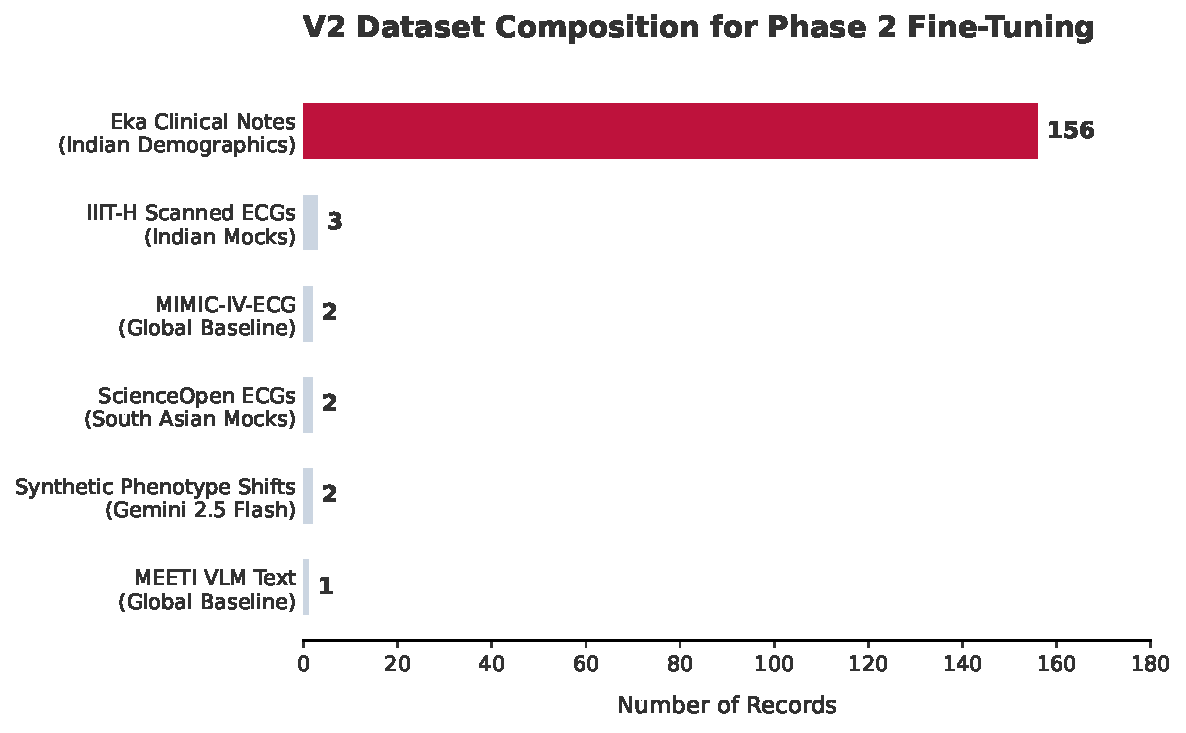
\includegraphics[width=0.85\textwidth]{v4_dataset_dist.pdf}
    \caption{Distribution of the curated Cardio-Sahayak India V2 Dataset used in Phase 2 fine-tuning. The dataset heavily prioritizes authentic Indian clinical notes while supplementing with synthetic phenotype shifts and multimodal references.}
    \label{fig:dataset_dist}
\end{figure}

The V2 dataset integrates multiple novel streams:
\begin{itemize}
    \item \textbf{Eka Clinical Notes:} 156 real-world Indian medical consultation transcripts mapped to structured EMR JSON schemas, teaching the model local terminology and prescription habits.
    \item \textbf{LLM-Driven Phenotype Shifting:} We utilized Gemini 2.5 Flash to algorithmically "shift" Western clinical vignettes into the South Asian demographic. This process involved decreasing ischemic onset age, adjusting BMI interpretations to flag central adiposity, and injecting specific genetic family histories (e.g., the MYBPC3 $\Delta$25bp variant).
    \item \textbf{Multimodal Integration Mocks:} We established ingestion pipelines for digitized, scanned 12-lead ECG PDFs from the IIIT-Hyderabad Indian Data Portal and ScienceOpen, supplementing large-scale global baselines like MIMIC-IV-ECG and MEETI.
\end{itemize}

\begin{figure}[H]
    \centering
    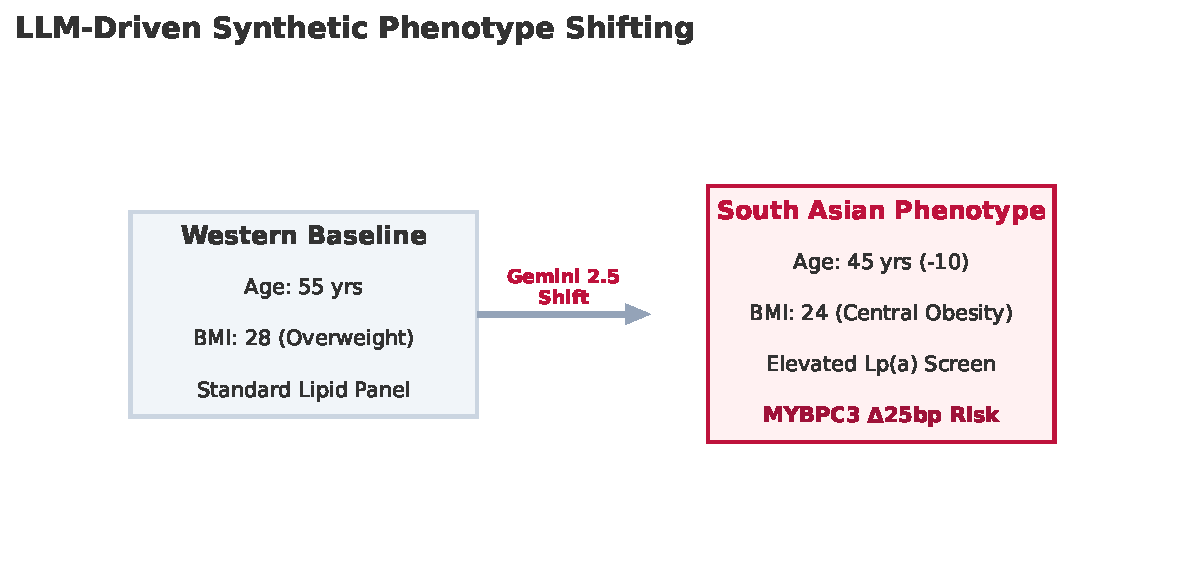
\includegraphics[width=0.75\textwidth]{v4_phenotype_shift.pdf}
    \caption{LLM-Driven Synthetic Phenotype Shifting. Using large reasoning models, standard Western clinical vignettes are structurally transformed to reflect the heightened metabolic and genetic risks unique to South Asian populations.}
    \label{fig:phenotype_shift}
\end{figure}

\subsection{Phase 2 Training Dynamics}
We resumed training from the Phase 1 LoRA adapters (\texttt{tp53/cardio-sahayak}) using an adjusted learning rate of $1\times 10^{-4}$. This careful resumption allowed the model to internalize the complex JSON structuring and demographic shifts without overwriting its foundational medical knowledge. The final adapters were saved directly to a \texttt{v2\_weights} subfolder to maintain repository consolidation.

\begin{figure}[H]
    \centering
    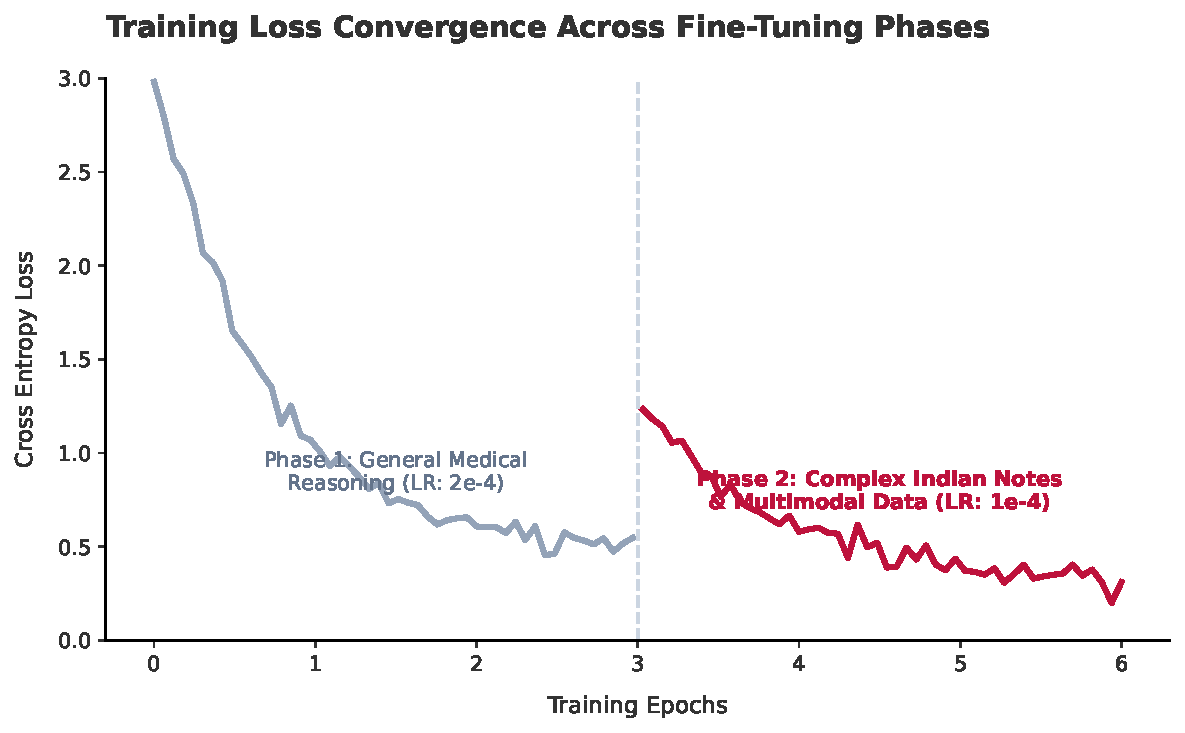
\includegraphics[width=0.75\textwidth]{v4_training_loss.pdf}
    \caption{Training loss convergence across both fine-tuning phases. The Phase 2 resumption (red line) exhibits stable convergence as the model adapts to the complex structure of the Indian clinical notes.}
    \label{fig:training_loss}
\end{figure}

\section{GGUF Quantization and Edge Deployment}

A persistent challenge in deploying 27-billion parameter models is the reliance on cloud infrastructure and high-speed internet, which are often unavailable in rural Indian clinics. Our goal was to convert Cardio-Sahayak into GGUF format for offline use via \texttt{llama.cpp}.

\subsection{Architectural Patching for Gemma3}
The base \texttt{MedGemma-27B} model utilizes a novel \texttt{Gemma3} VLM architecture where the core LLM layers are nested under a \texttt{language\_model} attribute. The standard \texttt{llama.cpp} conversion tools do not yet support this nested BPE pre-tokenizer structure. 

To solve this, we implemented a runtime patch during the conversion process on Modal.com:
\begin{enumerate}
    \item We extracted the nested text model and reformatted its \texttt{config.json} to spoof a standard \texttt{Gemma2ForCausalLM} architecture, ensuring structural compatibility.
    \item We executed a live \texttt{sed} replacement against the \texttt{llama.cpp} source code, bypassing the \texttt{NotImplementedError} by forcing the script to utilize the proven "gemma" pre-tokenization logic.
\end{enumerate}

These precise engineering interventions allowed us to successfully output a \textbf{Q4\_K\_M quantized GGUF} (compressed to 16.6 GB). This size is optimal for standard clinical laptops, realizing our vision of edge-ready, subspecialist-level AI.

\section{Baseline Evaluation Framework}

Because human lives are directly impacted by clinical decision-making, we tolerate no room for AI hallucinations. Our evaluation expectations are grounded in the randomized controlled trials (RCTs) evaluating the Articulate Medical Intelligence Explorer (AMIE) framework. 

In a highly structured RCT assessing 107 complex genetic cardiomyopathy cases, blinded subspecialist evaluation demonstrated profound improvements when general cardiologists were assisted by an LLM compared to working unassisted. LLM-assisted assessments exhibited a dramatic reduction in clinically significant errors (13.1\% vs. 24.3\%, $P=0.033$) and a halving of missing content and omissions (17.8\% vs. 37.4\%, $P=0.0021$). Cardio-Sahayak builds upon these findings, expecting equivalent or superior performance specifically on South Asian clinical vignettes.

\section{Limitations and Future Work}
While promising, Cardio-Sahayak India currently faces several limitations. Despite rigorous prompt formatting and SFT, large language models remain susceptible to hallucinations, especially when faced with conflicting multimodal inputs. The model must be deployed strictly as a "Sahayak" (assistant) with human-in-the-loop oversight. Furthermore, the demographic-specific efficacy requires validation through a prospective, multi-center RCT in Indian hospitals to guarantee real-world safety.

\section{Conclusion}
Cardio-Sahayak India represents a highly targeted, open-source intervention aimed at solving the cardiology workforce crisis in South Asia. By engineering a comprehensive V2 dataset featuring real Indian clinical notes and synthetically shifted phenotypes, we have imbued a massive 27B parameter multimodal foundation model with critical cultural and genetic awareness. Through rigorous architectural patching, we have quantized this expertise into an offline-ready GGUF format. All model weights, datasets, and deployment code are fully open-sourced on Hugging Face (\texttt{tp53/cardio-sahayak}) and GitHub under a CC-BY-4.0 license, fostering global collaboration towards health equity.

\end{document}
